\documentclass[11pt]{article}

\usepackage{amsmath, amssymb, amsthm}
\usepackage{tikz}

\theoremstyle{plain}
\newtheorem{thm}{Theorem}[section]
\newtheorem*{thm*}{Theorem}
\newtheorem{prop}[thm]{Proposition}
\newtheorem{lem}[thm]{Lemma}
\newtheorem*{lem*}{Lemma}
\newtheorem{dfn}[thm]{Definition}
\newtheorem{cor}[thm]{Corollary}
\newtheorem{claim}[thm]{Claim}
\newtheorem{conj}[thm]{Conjecture}
\newtheorem{ques}[thm]{Question}
\newtheorem*{rem}{Remark}


\oddsidemargin  0pt
\evensidemargin 0pt
\marginparwidth 40pt
\marginparsep 10pt
\topmargin 0pt
\headsep 10pt
\textheight 8.2in
\textwidth 6.4in
\renewcommand{\baselinestretch}{1.1}

\newcommand{\codeg}{\text{codeg}}
\newcommand{\BBE}{\mathbb{E}}
\newcommand{\BFP}{\mathbf{P}}
\usepackage{amsmath}
\usepackage{amsthm}
\usepackage{amssymb}
\usepackage{mathtools}
\usepackage{hyperref}
\usepackage{url}





\usepackage{graphicx}
\usepackage{caption}
\usepackage{subcaption}

\def\eQb#1\eQe{\begin{eqnarray*}#1\end{eqnarray*}}
\def\eQnb#1\eQne{\begin{eqnarray}#1\end{eqnarray}}
\providecommand{\e}[1]{\ensuremath{\times 10^{#1}}}
\providecommand{\pb}[0]{\pagebreak}
\DeclarePairedDelimiter\ceil{\lceil}{\rceil}
\DeclarePairedDelimiter\floor{\lfloor}{\rfloor}

\newcommand{\E}{\mathrm{E}}
\newcommand{\Var}{\mathrm{Var}}
\newcommand{\Cov}{\mathrm{Cov}}

\def\Qb#1\Qe{\begin{question}#1\end{question}}
\def\Sb#1\Se{\begin{solution}#1\end{solution}}


\newtheoremstyle{quest}{\topsep}{\topsep}{}{}{\bfseries}{}{ }{\thmname{#1}\thmnote{ #3}.}
\theoremstyle{quest}
\newtheorem*{definition}{Definition}
\newtheorem*{theorem}{Theorem}
\newtheorem*{lemma}{Lemma}
\newtheorem*{question}{Question}
\newtheorem*{preposition}{Preposition}
\newtheorem*{exercise}{Exercise}
\newtheorem*{challengeproblem}{Challenge Problem}
\newtheorem*{solution}{Solution}
\newtheorem*{remark}{Remark}
\usepackage{verbatimbox}
\usepackage{listings}
\usepackage{mathrsfs}
\date{}
\title{\vspace{-0.7cm}
Diff Geo II: Problem Set VI}

\author{
Youngduck Choi 
\thanks{Department of Mathematics, Courant Institute of Mathematical Sciences, 
yc1104@nyu.edu; If you find an error and want to share with me, 
you can reach me via email.
}}

\begin{document}

\maketitle

\begin{abstract}
This work contains solutions for the problem set VI.
\end{abstract}


\begin{question}[1-1]
\hfill
\begin{figure}[h!]
  \centering
    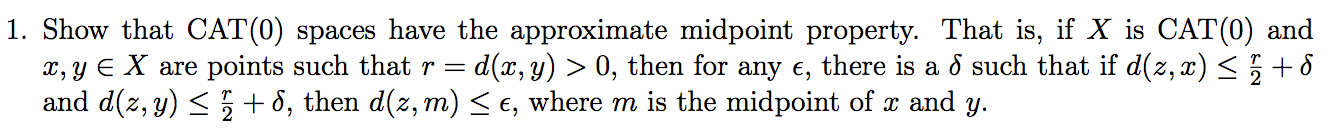
\includegraphics[width=0.7\textwidth]{dg2-s6-p1.png}
\end{figure}
\end{question}
\begin{solution} \hfill \\
Consider $\angle_m(z,x)$ and $\angle_m(z,y)$ such that 
$d(z,x) \leq \dfrac{r}{2} + \delta$ for some $\delta > 0$. 
As $X$ is non-positively curved,
we can assume without loss of
generality that $\angle_m(z,x) \geq \frac{\pi}{2}$. Then,  
the angle at $\bar{m}$ for the comparison triangle $\bar{\triangle}(m,z,x)$ is
greater than equal to $\frac{\pi}{2}$.  
Hence, by the Cosine law, 
\eQb
(\frac{r}{2})^2 + d(m,z)^2 &=& d(x,m)^2 + d(m,z)^2 \\ 
&\leq& d(z,x)^2 \leq (\dfrac{r}{2} + \delta)^2 
\eQe
so
\eQb
d(m,z)^2 &\leq& r\delta + \delta^2.
\eQe
Therefore, as $r > 0$ is fixed, for any given $\epsilon >0$,
we can choose $\delta > 0$ small enough,
$d(m,z) \leq \epsilon$, and we are done. \hfill $\qed$ 


\end{solution}

\newpage

\begin{question}[1-2]
\hfill
\begin{figure}[h!]
  \centering
    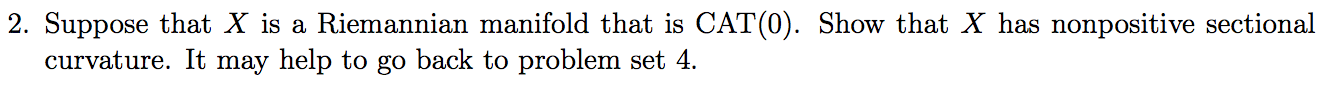
\includegraphics[width=0.7\textwidth]{dg2-s6-p2.png}
\end{figure}
\end{question}
\begin{solution} \hfill \\
In this problem, we show that in the Riemmannian category, 
if the Riemannian distance, induced by the Riemannian metric is a metric, which satisfies
the curvature condition of bounded above by $0$ in the sense of Alexandrov, then
the sectional curvature of the Riemannian metric is everywhere bounded above by $0$.
Hence, we see that the theory of Alexandrov spaces generalizes the 
sectional curvature part of Riemannian geometry in a particular way
by focusing on the structure of sectional curvature having uniform bound from 
above. We now proceed with the proof. Let $x \in M$, and $U$, $V \in T_x M$, such that
$U$ and $V$ are orthonormal. Then, let $K$ be the sectional curvature of the plane,
spanned by $U$ and $V$, in $T_x M$. Via normal coordinates, for all $t$ small enough,
we have two unique geodesics $t \mapsto \exp_x(tU)$ and $t \mapsto \exp_x(tV)$
such that the tangent vectors at $x$ at $t = 0$ are $U$ and $V$ respectively. Set
$a(t) = d(\exp_x(tU),\exp_x(tV))$. From the homework set $4$, squaring the expression
in the problem $2$ gives in normal coordinate,
\eQnb
a(t)^2 &=& 2t^2 - \dfrac{K}{6}t^4 + O(t^5) \label{eq:1-2-1}.
\eQne 
Now, consider a geodesic triangle(straight lines) in $\mathbb{R}^2$ with side lengths $t$,
and orthogonal. Then, we claim that
\eQnb
a(t)^2 \geq s(t)^2 = 2t^2 \label{eq:1-2-2} 
\eQne
where the $s(t)$ is the length of the third side on the Euclidean triangle. 
Clearly, the last equality
is from the Pythagorean theorem, and in view of~\eqref{eq:1-2-1} and considering
$t$ small, it suffices to show~\eqref{eq:1-2-2} to conclude that $K \leq 0$. 
From the solution to the problem 3, we can deduce that the Alexandrov angle
between sides of any geodesic in $X$ with distinct vertices is less than or equal
to the angle between the corresponding sides of the comparison triangle in $\mathbb{R}^2$
. Now, as $d(\exp_x(tV), x) = t$ and $d(\exp_x(tU),x) = t$ by a property of 
normal neighborhoods, and by the Cosine law, we see that 
\eQb
a(t)^2 &=& d(\exp_x(TU), \exp_X(tV)) \geq s(t)^2 = 2t^2.
\eQe 
Since $K$ was arbitrary, we are done. \hfill $\qed$
 
\end{solution}

\newpage

\begin{question}[1-3]
\hfill
\begin{figure}[h!]
  \centering
    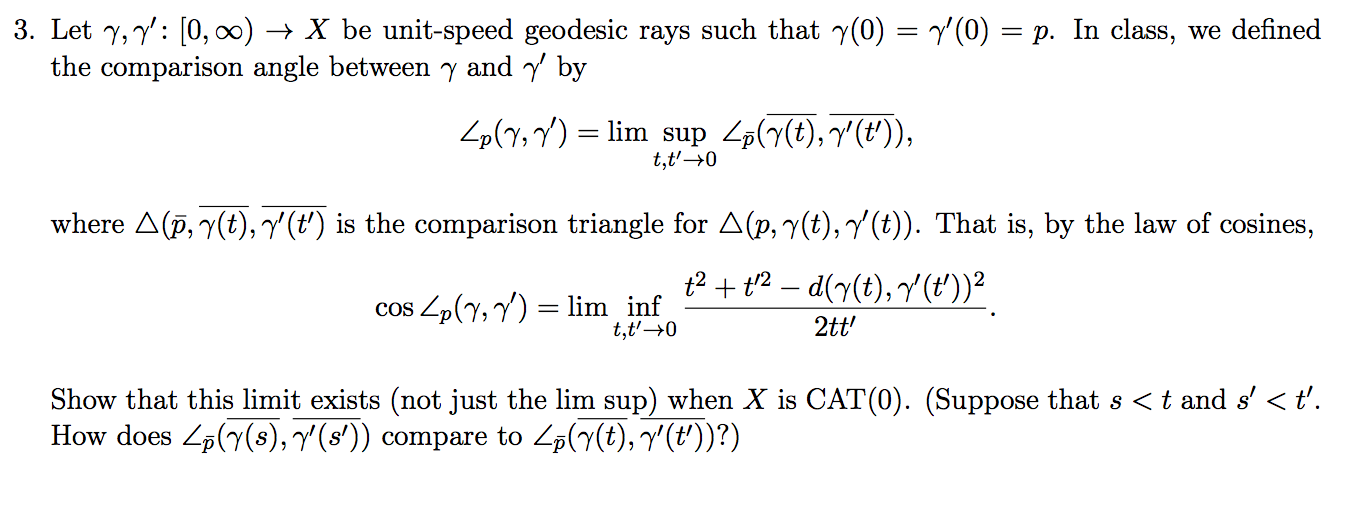
\includegraphics[width=0.7\textwidth]{dg2-s6-p3.png}
\end{figure}
\end{question}
\begin{solution} \hfill \\
The key idea in this proof is that the lines on the compared triangle have the
same length as the original length, as opposed to general lines inside the compared
triangle.
With the given set up, it suffices to show that
\eQb
\angle_{\bar{p}} (\overline{\gamma(s)}, \overline{\gamma(s')}) &\leq&  
\angle_{\bar{p}} (\overline{\gamma(t)}, \overline{\gamma(t')}), 
\eQe
since monotonicity of the limit will show that the a priori $\limsup$ is in fact $\lim$.
Denote compared triangles on $\mathbb{R}^2$ as $\bar{\triangle}(p,\gamma(s),\gamma(s'))$,
and  $\bar{\triangle}(p,\gamma(t),\gamma(t'))$. Now, observe that by the first 
comparison, 
\eQb
d(\overline{\gamma(s)}_1, \overline{\gamma(s')}_1) &=& 
d(\gamma(s), \gamma(s')) 
\eQe 
and from the second comparison
\eQb
d(\overline{\gamma(s)}_2, \overline{\gamma(s')}_2) &\geq&  
d(\gamma(s), \gamma(s'))
\eQe
so
\eQb
d(\overline{\gamma(s)}_2, \overline{\gamma(s')}_2) &\geq&  
d(\overline{\gamma(s)}_1, \overline{\gamma(s')}_1). 
\eQe
Then, by the Cosine law on the Euclidean space (recall that all lines on the compared
triangle have the same length as the original triangle, as oppposed to lines
inside the compared triangle in general, and cosine is decreasing as the angle increases
to $\pi$)
\eQb
\angle_{\bar{p},2}(\overline{\gamma(t)}, \overline{\gamma(t')}) &=& 
\angle_{\bar{p},2}(\overline{\gamma(s)}, \overline{\gamma(s')}) \\
&\geq&
\angle_{\bar{p},1}(\overline{\gamma(s)}, \overline{\gamma(s')}) 
\eQe
where we denoted the comparison angle explicitly with respect to the first and the
second triangle. Hence, we are done. \hfill $\qed$
\end{solution}


\end{document}

